\section{Task 3.1}
\subsection{Dataset Preparation}
For the first task of the project (also for task 3.3) a preprocessing of the given dataset has been carried out in the \textsc{Matlab} file \verb*|dataset_preparation.m|.\\

First of all a \textbf{cleaning process} has been done in order to remove Non-Numeric data or Infinite numbers in the dataset.\\
Then a procedure of \textbf{outliers removal} has been carried out: to do so, some experiments have been done out with the way to perform outlier removal. Two parallel experiment were made and at the end the \textit{median} method has been selected as optimal by comparing the neural network regression performance. \\

The next step was \textbf{data balancing}, since the outputs can assume only seven different values for both arousal and valence. In order to obtain the latter point, \textbf{data augmentation} has been performed by multiplying selected data by a random number between \([0.95, 1.05]\).\\
The data to augment was obtained as follows: from the indexes of the least common class for arousal(valence) were removed the indexes of the most common class for valence(arousal). Then, the resulting indexes were lowered if by adding them to the least common class, the result would go beyond the most common class of that type. This last operation permitted to obtain a certain degree of "convergence" of the whole process, which was repeated different times. \\
In the following image are presented the results of data augmentation:  
\begin{figure}[H]
	\centering
	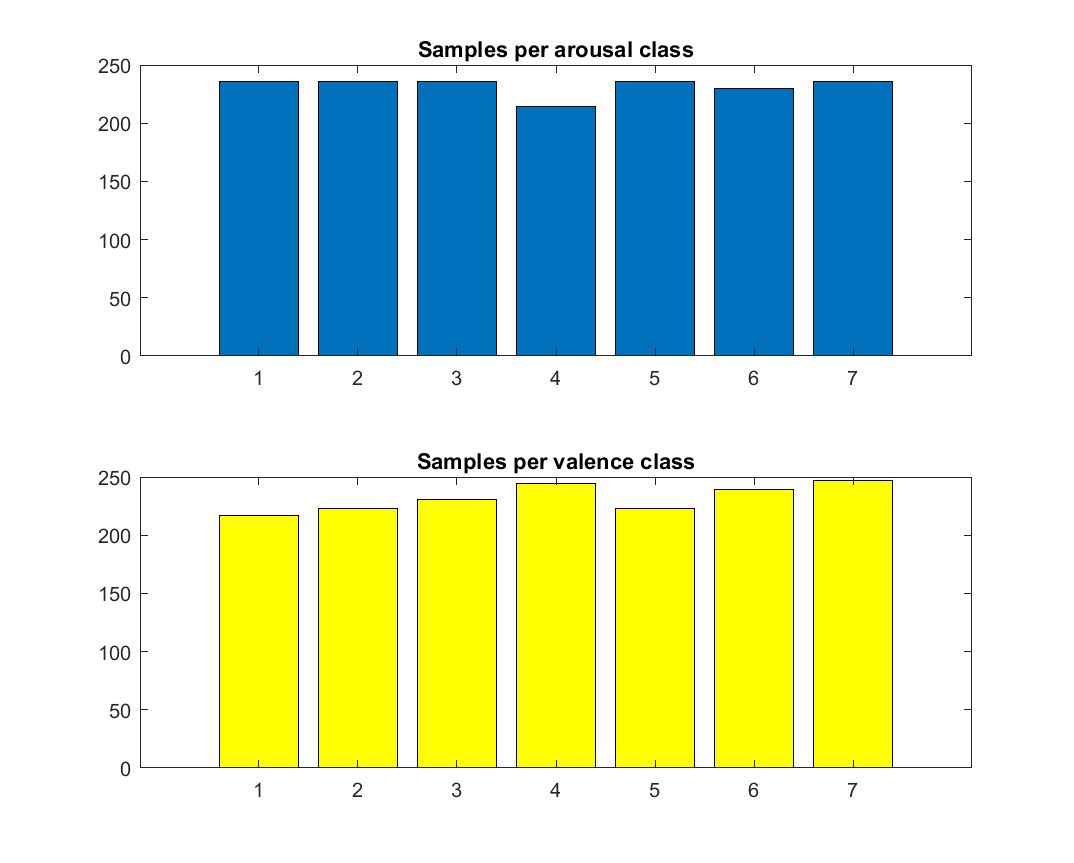
\includegraphics[width=0.7\linewidth]{img/bar_plot_arousal_valence.png}
	\caption{Data Balancing results}
\end{figure}
The last step of the process was the \textbf{feature selection step}: firstly, data has been divided through an \textbf{holdout partition} into training and test data (the latter will be used to assess the final performance of the net); secondly, through the \verb|sequentialfs| function the features have been extracted from the training data by exploiting the following function:


\begin{lstlisting}[language=Matlab]
function err = fun2(x_train, t_train, x_test, t_test)
	% Around 1000 samples for training
	% 1 input neuron, 1 output neuron
	% Chose 60 neurons for the hidden layer of the fitnet
	
	net = fitnet(60);
	net.trainParam.showWindow=0;
	xx = x_train';
	tt = t_train';
	net = train(net, xx, tt);
	y=net(x_test'); 
	err = perform(net,t_test',y);
end
\end{lstlisting}

For what concerns the \textbf{number of hidden neurons}, the following formula has been used in order to prevent over-fitting by determining a upper bound for neurons on hidden layer:

\begin{equation}
	N_{h} = \frac{N_{s}}{\alpha * (N_{i} + N_{o})}
\end{equation}

Where \(N_{h}\) represents the upper bound for hidden neuron, \(N_{s}\) the number of samples, \(N_{i}\) the number of input neurons, \(N_{o}\) the number of output neurons and \(\alpha\) a scaling factor between 2 and 10. \\
The method of matching the number of weights as 5 or 10 times the number of samples was not used, since it would imply an higher number of neurons in the fun2 function and the general feature selection process would take much longer computational effort.\\

The \verb|sequentialfs| has been ran \textbf{100 times} for giving statistical meaning to results and at the same time limit the computational effort of the machine. Each feature selected has been counted in a counter vector and at the end this vector has been sorted in descending order in order to obtain the list of most important features. Two different sorted vector were obtained, one for arousal and another for valence.
 
\subsection{MLP Training}

After loading the results of the feature selection process, some \textbf{experiments for finding the best architecture} for MLPs in terms of pure fitting of arousal and valence has been carried out:
by \textbf{changing the number of neurons} (i.e for the first hidden layer around the interval [5, 120], trying to minimize this number as soon as good results started to appear), by changing the training function, by modifying the maximum number of \textbf{validation fails}, the \textbf{number of epochs} and by adding some momentum and so on.
In general good performance (in terms of regression) were obtained by using \textbf{only one hidden layer} and a similar number of neurons used in the feature selection process while other parameters didn't seem to influence greatly the regression of the MLP. \\
For what concerns the best architecture for MLPs and the related regression performance (w.r.t. the test set obtained from the holdout partition before the feature selection), in the following are presented those results:
\begin{figure}[H]
	\centering
	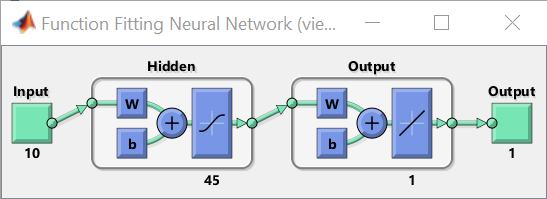
\includegraphics{img/arousal_mlp_45.png} 
	\caption{MLP Structure for arousal}
\end{figure}
\begin{lstlisting}[language=Matlab]
	% Configuration for training of the MLP for arousal 
	% (non present fields are the default ones)
	mlp_net_arousal.trainParam.lr = 0.1; 
	mlp_net_arousal.trainParam.epochs = 100;
	mlp_net_arousal.trainParam.max_fail = 10;
\end{lstlisting}

\begin{figure}[H]
	\centering
	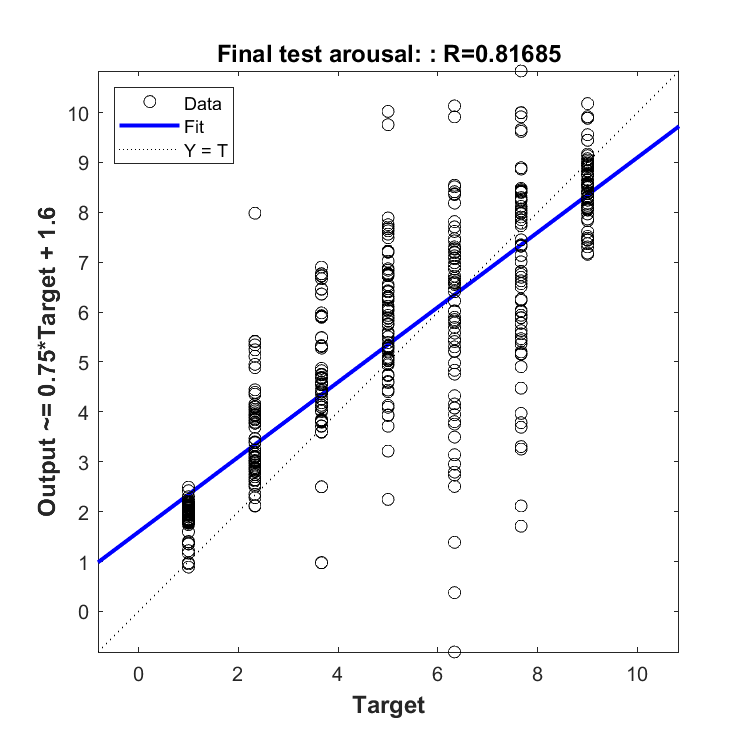
\includegraphics[width=0.5\linewidth]{img/arousal_mlp_45_regression_with_testset.png} 
	\caption{Regression for arousal}
\end{figure}
\begin{figure}[H]
	\centering
	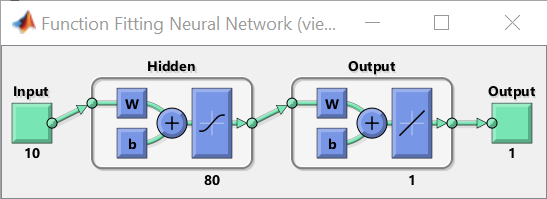
\includegraphics{img/valence_mlp_80.png} 
	\caption{MLP Structure for valence}
\end{figure}
\begin{lstlisting}[language=Matlab]
	% Configuration for training of the MLP for valence
	% (non present fields are the default ones)
	mlp_net_valence.trainParam.lr = 0.1; 
	mlp_net_valence.trainParam.epochs = 100;
	mlp_net_valence.trainParam.max_fail = 15;
\end{lstlisting}

\begin{figure}[H]
	\centering
	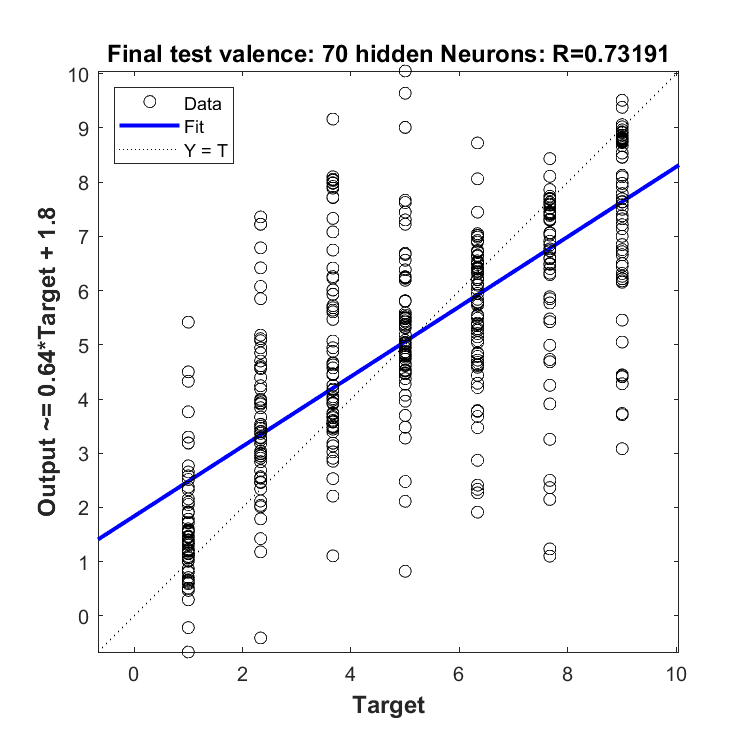
\includegraphics[width=0.5\linewidth]{img/valence_mlp_80_regression_with_testset.png} 
	\caption{Regression for valence}
\end{figure}
As we can see better results were obtained with the MLP for the arousal. An interesting observation can be inferred by watching the result of the training process: data was split another time into a training set, a test set and a validation set (for early stopping) with the following results in term of regression:

\begin{figure}[H]
	\centering
	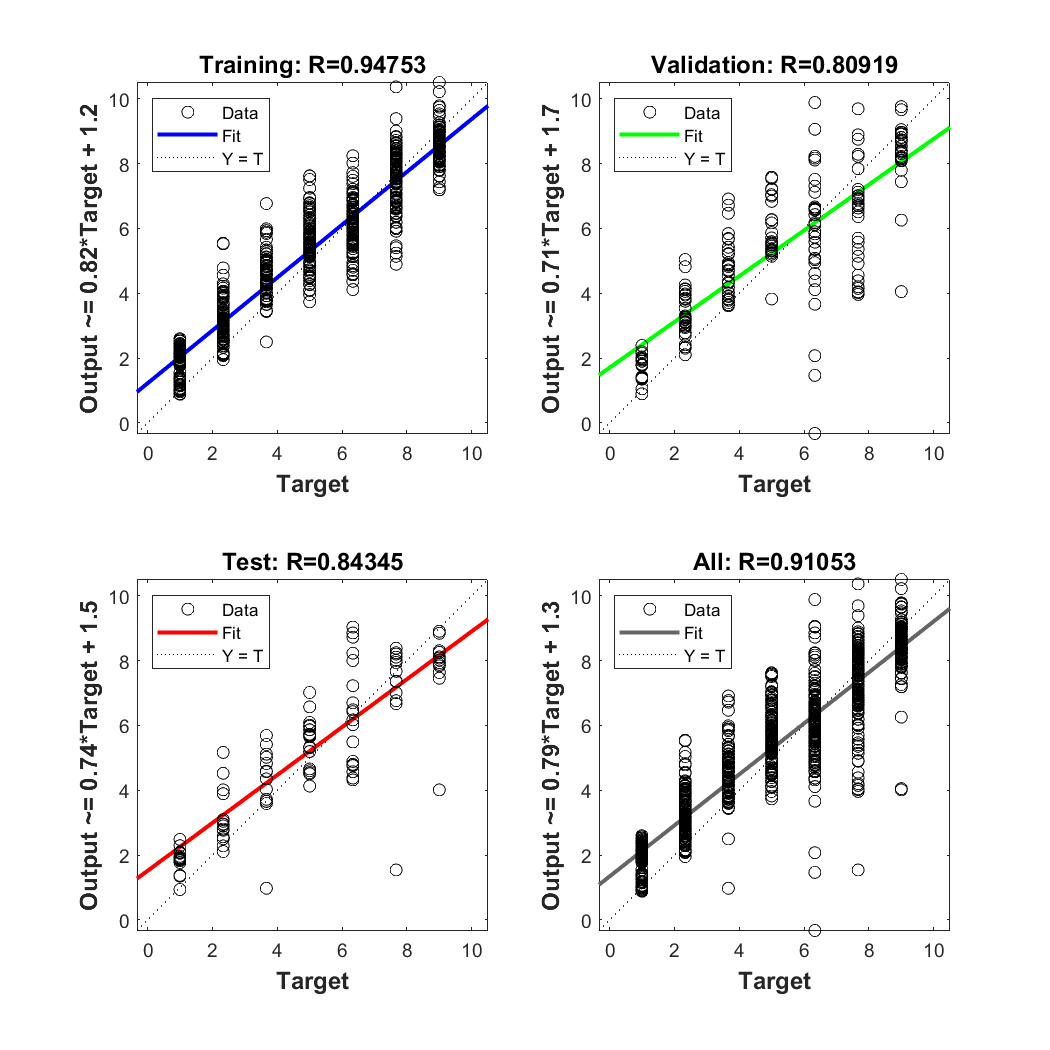
\includegraphics[width=0.7\linewidth]{img/arousal_mlp_45_regression.png} 
	\caption{MLP regression results after training}
\end{figure}

In this case the test set has a slightly higher R-squared w.r.t. the test-set obtained at the beginning with the holdout partition. In fact those samples has been given in input to the \verb|sequentialfs| giving a positive bias for the regression of the data.

\subsection{RBF Training}
For what concerns RBF networks, the training process adopted was simpler since there were less degrees of freedom with the \verb|newrb| function. In particular experiments were carried out by changing values of the \textbf{spread} in order to obtain the best possible result in terms of regression w.r.t. the test set obtained by the holdout partition. The final parameters were the following:
\begin{lstlisting}[language=Matlab]
	%Parameters for training the RBF for arousal
	spread_ar = 1.07;
	goal_ar = 0;
	K_ar = 1200; %Maximum number of neurons
	Ki_ar = 100; %Step (default was 50, to make the process quicker it was increased)
\end{lstlisting}

\begin{figure}[H]
	\centering
	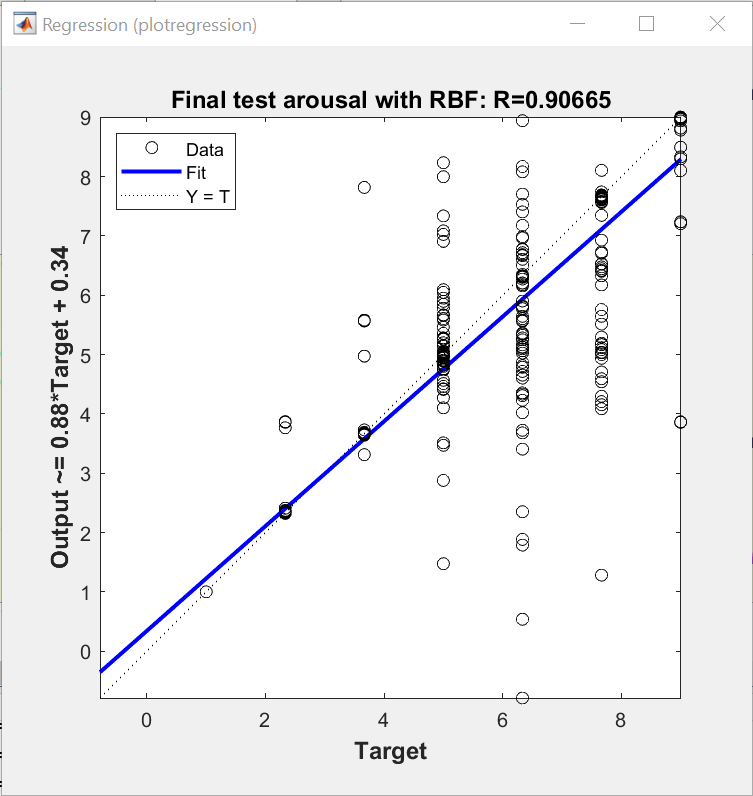
\includegraphics[width=0.5\linewidth]{img/arousal_rbf_1_3.png}
	\caption{Regression of RBF for arousal with Test Set}
\end{figure}

\begin{lstlisting}[language=Matlab]
	%Parameters for training the RBF for valence
	spread_va = 0.7;
	goal_va = 0;
	K_va = 1200;
	Ki_va = 100;
\end{lstlisting}

\begin{figure}[H]
	\centering
	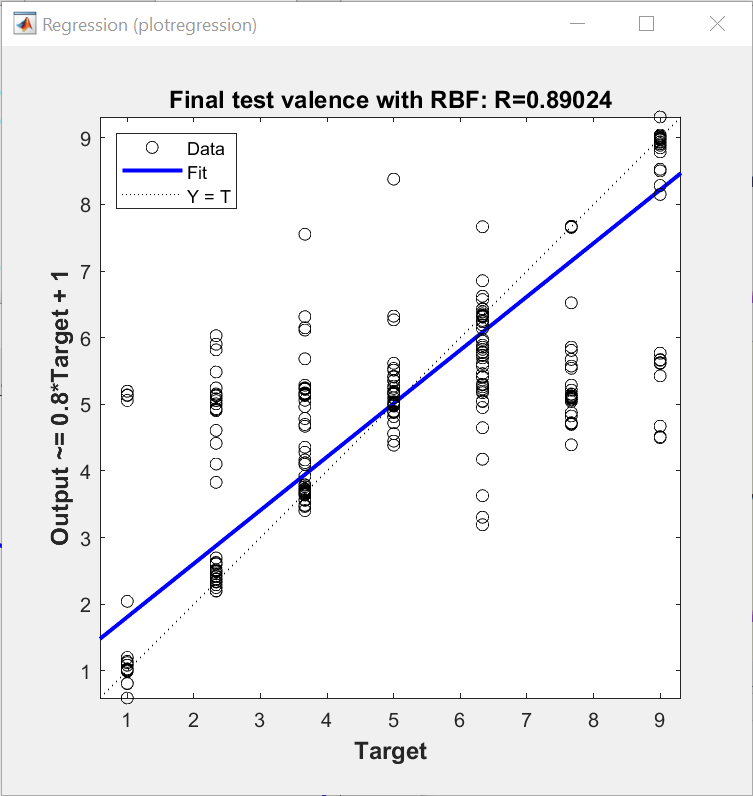
\includegraphics[width=0.5\linewidth]{img/valence_rbf_0_7.png}
	\caption{Regression of MLP with Test Set}
\end{figure}
